\chapter{Estructura electrònica dels àtoms i propietats periòdiques}

\section{L'estructura electrònica dels àtoms}
\subsection{Radiació d'un cos negre}
\begin{figure}[h]
\centering
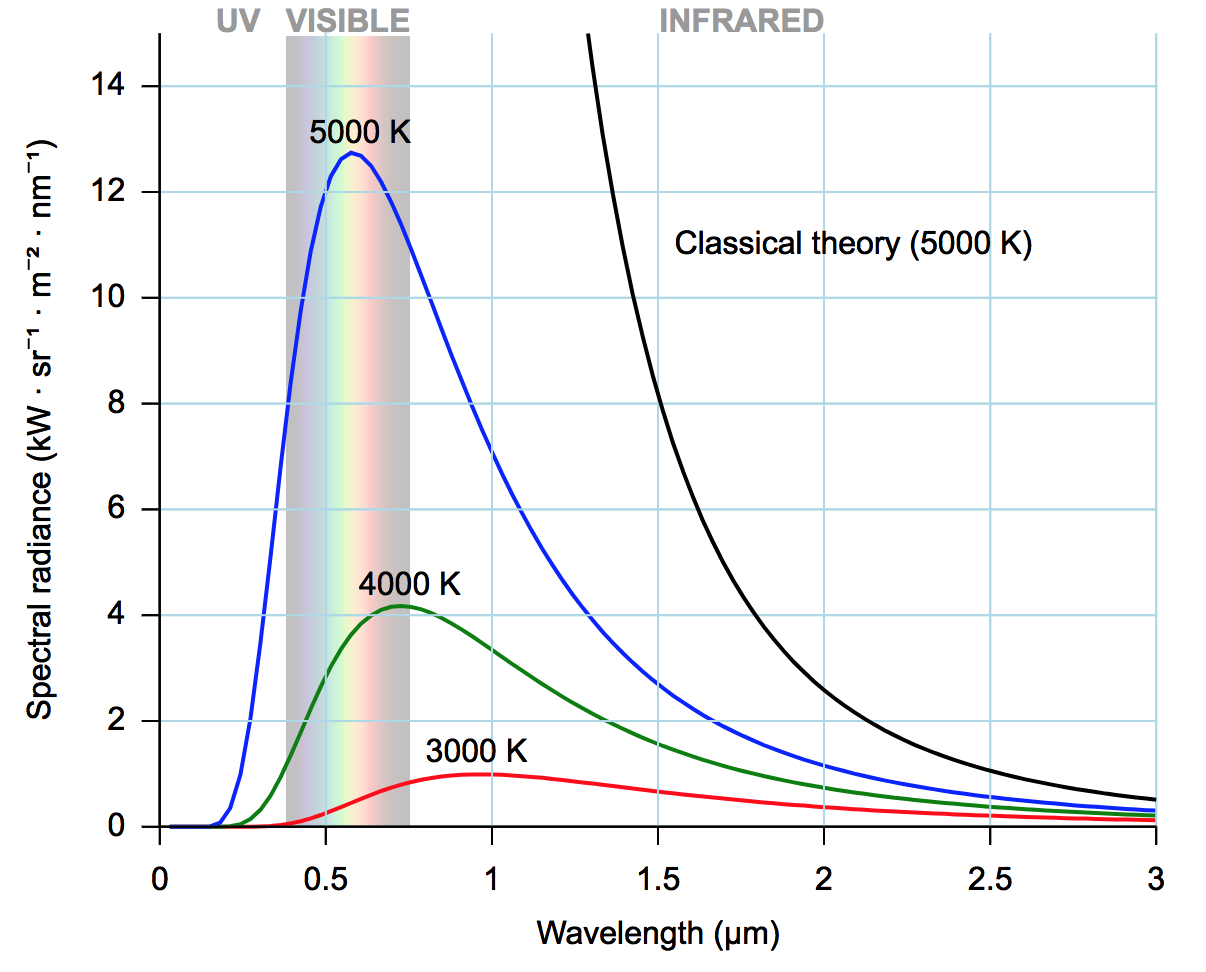
\includegraphics[scale=0.5]{blackbody.png}
\caption{Distribució de freqüències de radiació emeses per un cos negre}
\label{fig:blackbody}
\end{figure}
Rayleigh (Juny 1900). Radiació contínua $\lambda \nu = c$:
\[
R(\nu)=\frac{2 \pi k T}{c^2} \nu^2
\]
Planck (Octubre-Desembre 1900). Radiació en paquets $h\nu$ (\textit{quantum}):
\[
R(\nu)=\frac{c_1 \nu^3}{e^{c_2 \nu T} -1}=\frac{2\pi h \nu^3}{c^2} \frac{1}{e^{h\nu/kT}-1}
\]
\subsection{Efecte fotoelèctric i experiment de Rutherford}
\begin{figure}[h]
\centering
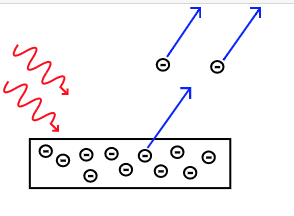
\includegraphics[scale=1.5]{photoelect.png}
\caption{Efecte fotoelèctric}
\label{fig:photoelect}
\end{figure}
Lenard (Nobel 1905, raigs catòdics):
\begin{enumerate}
\item La freqüència llindar $\nu_0$ d'emissió depèn de cada metall
\item més llum, més electrons, però amb la mateixa energia cinètica
\item Més freqüència de radiació més energia cinètica electrons
\end{enumerate}
Einstein (1905):
\[
E_{fotó}=h \nu
\]
\[
h\nu = W + 1/2 m v^2
\]
Però per explicar-ho implicava introduir el concepte de dualitat ona-corpuscle.

Des dels experiments de Thomson amb raigs catòdics (1897) i Milikan (1909) es sabia que els àtoms estaven formats per càrregues positives i negatives, però es pensava que tenien forma esfèrica amb els electrons al seu interior.
\begin{figure}[h]
\centering
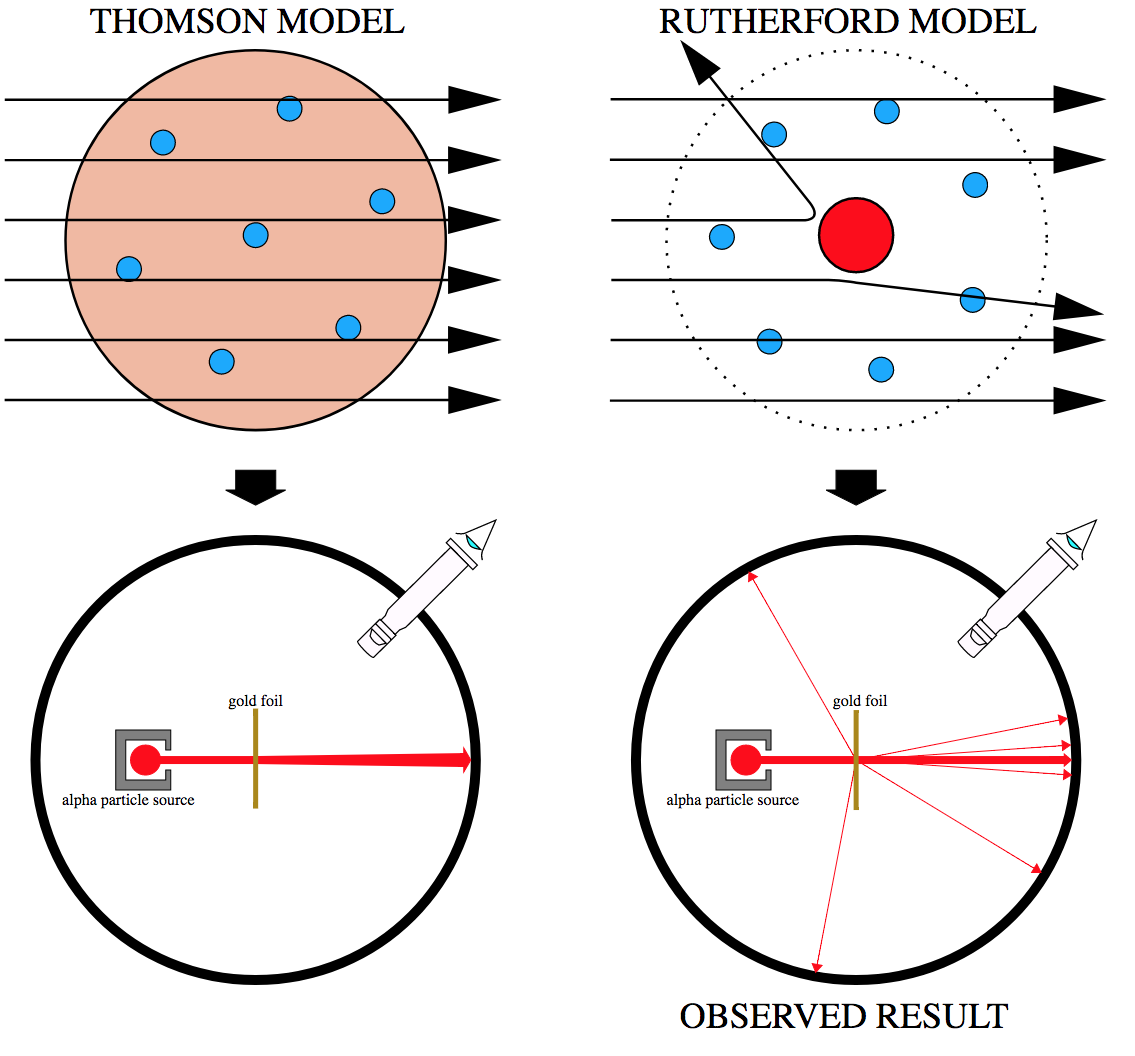
\includegraphics[scale=0.5]{Rutherford.png}
\caption[Model de Rutherford]{La figura de l'esquerra mostra com haurien de travessar una placa metàl·lica partícules $\alpha$ segons el model de Thomson, A la dreta de la figura apareix l'explicació del comportament experimental real segons el model de Rutherford.}
\label{fig:Rutherford}
\end{figure}
Rutherford (1911) va mostrar que l'àtom no podia ser una esfera uniforme com la predita. Va mostrar que fent impactar partícules $\alpha$ (nuclis d'àtoms d'heli; per tant, amb càrrega +2 i massa 4) sobre una placa fina de metall es produïa ampla difracció d'un nombre petit de partícules i n'hi havia moltíssimes que travessaven la placa sense cap desviació o ben poca. Això implicava que els àtoms havien d'estar formats per una massa central altament carregada positivament i havien de tenir un volum molt més gran per tal que les partícules majoritàriament travessessin la placa (Figura \ref{fig:Rutherford})\footnote{\linkurl{https://commons.wikimedia.org/wiki/File:Geiger-Marsden_experiment_expectation_and_result.svg}}.

\subsection{Àtom de Bohr}
\begin{figure}[h]
\centering
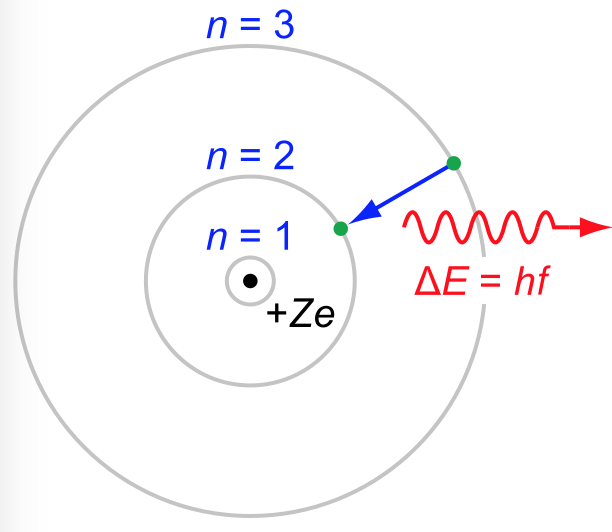
\includegraphics[scale=0.7]{Bohr.png}
\caption{Model de l'àtom de Bohr}
\label{fig:Bohr}
\end{figure}
Balmer, Rydberg (1885-1910); freqüències espectrals per a l'àtom d'hidrogen:
\begin{equation}
\frac{\nu}{c}=\frac{1}{\lambda}=R\left( \frac{1}{n_b^2}-\frac{1}{n_a^2}\right)
\label{eq:rydberg}
\end{equation}
\[
n_b=1,2,3,\dots; \; n_a=2,3,4,\dots; n_a>n_b
\]
on R=109677.6 cm$^{-1}$.

Bohr (1913):
\begin{enumerate}
\item estats estacionaris de l'àtom d'H
\item un estat estacionari no emet energia electromagnètica
\item l'emissió entre estats és igual a un fotó: $E_a-E_b=h\nu$.
\end{enumerate}
A partir de l'Eq. \ref{eq:rydberg} i aquest resultat, es pot veure que l'energia dels estats estacionaris del H ve donada per $E=-Rhc/n^2$ amb $n=1,2,3,\dots$. I va afegir dos postulats més al seu model:
\begin{enumerate}
\item l'electró de l'estat estacionari es mou en un cercle de radi determinat
\item hi ha una relació entre el radi d'aquestes òrbites i la seva energia $mvr=\frac{nh}{2\pi}$
\end{enumerate}
A partir d'aquí, va deduir una energia per a cada nivell d'energia:
\[
E=\frac{-2\pi^2 m e'^4}{h^2n^2}
\]
i $R=\frac{-2\pi^2 m e'^4}{h^3c}$. El resultat concorda amb l¡experiment i dóna els nivells correctes de les energies de l'àtom de Bohr, però els dos darrers postulats són totalment falsos i va ser el 1926 quan Schrödinger va formular la seva equació de la mecànica quàntica que superava el model de Bohr.

\subsection{Hipòtesi de de Broglie i principi d'incertesa}
El 1923, de Broglie va formular la hipòtesi de que la matèria, com la llum, també tenia naturalesa dual ona-corpuscle. 
Això explicaria el rerafons del model de Bohr: els electrons mostraven nivells d'energia quantitzats.
En el cas de la llum, Einstein havia arribat a que la relació entre la longitud d'ona i la massa d'un fotó era $\lambda=h/mc$. De Broglie va aplicar el mateix raonament a una partícula de massa $m$ i velocitat $v$: $\lambda=h/mv$.

A partir de considerar aquesta hipòtesi i la natura dual de les partícules, es pot arribar a veure que el producte de les incerteses en el càlcul de la posició i el moment lineal estan relacionades per $\Delta x \Delta p_x \geq h$, o principi d'incertesa de Heisenberg (1927).

\subsection{Mecànica quàntica}

Descrita per Heisenberg, Born i Jordan (1925) i per Schrödinger (1926). 

La mecànica clàssica és determinista, mentre que la quàntica és probabilística (pel principi d'incertesa de Heisenberg). L'Estat d'un sistema es determina per la seva funció d'estat $\Psi$, que és una funció de les coordenades de les partícules i del temps:
\begin{eqnarray}
-\frac{\hbar}{i} \frac{\partial \Psi}{\partial t}&=&-\frac{\hbar^2}{2m_1}\left(\frac{\partial^2\Psi}{\partial x_1^2}+\frac{\partial^2\Psi}{\partial y_1^2}+\frac{\partial^2\Psi}{\partial z_1^2} \right)-\\
 & & \cdots -\frac{\hbar^2}{2m_n}\left(\frac{\partial^2\Psi}{\partial x_n^2}+\frac{\partial^2\Psi}{\partial y_n^2}+\frac{\partial^2\Psi}{\partial z_n^2} \right) + V \Psi
\end{eqnarray}
on $\hbar=h/2\pi$, $i=\sqrt{-1}$, $m_1,\dots , m_n$ són les masses de les $n$ partícules de coordenades $x_i,y_i,z_i$ i $V$ és l'energia potencial del sistema.

El que ens interessa ara mateix és saber que la funció d'estat ens informa sobre l'estat del sistema.
A partir d'ella ho podem saber tot del sistema. El problema és trobar-la...

Per fer un cas senzill pensem en un sistema en el què l'energia potencial sigui independent del temps, com succeeix en un pàtom o una molècula aïllats. En aquest cas, l'equació es redueix a (per a una sola partícula)
\[
-\frac{\hbar^2}{2m}\frac{d^2 \psi(x)}{dx^2}+V(x)\psi(x)=E\psi(x)
\label{Eq:Schr1x}
\]
on $\psi$ és la funció d'ona del sistema.
\begin{figure}[h]
\centering
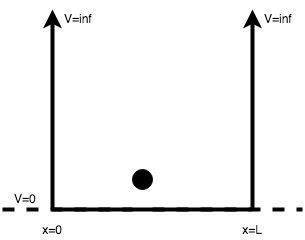
\includegraphics[scale=0.6]{ParticulaCaixa.png}
\caption{Partícula en una caixa unidimensional de potencial $V=0$ entre $x=0$ i $x=L$ i $V=\infty$ en qualsevol altre posició}
\label{fig:ParticulaCaixa}
\end{figure}
\begin{mdframed}[backgroundcolor=gray!30,frametitle=Partícula en una caixa]
Un dels sistemes més simples per als quals l'Eq. \ref{Eq:Schr1x} es pot solucionar és el cas d'una partícula en una caixa unidimensional de parets infranquejables i impenetrables.
Considerem una partícula de massa $m$ que es mou amb una energia $E$ positiva al llarg de l'eix $X$ entre $x=0$ i $x=L$ (Figura \ref{fig:ParticulaCaixa}).
A partir de l'Eq. \ref{Eq:Schr1x} obtenim, per a aquest sistema:
\[
-\frac{}{2m}\frac{d^2 \psi}{dx^2}+V\psi(x)=E\psi
\]
Ens adonem que per a la regió $0\leq x \leq L$, on $V=0$, podem escriure:
 \[
\frac{d^2 \psi}{dx^2}=-\frac{2mE}{\hbar^2}\psi
\label{Eq:PC1}
\]
Com sabem, la segona derivada d'una funció $\psi$ ens dona informació qualitativa sobre la seva corbatura. En aquest cas veiem que quan la $\psi$ sigui negativa la seva corbatura serà positiva, i a l'inrevés. La funció $\sin(x)$ és un exemple d'aquest tipus de funció. De fet, $\psi=A \sin(bx)$ és una solució de l'Eq. \ref{Eq:PC1}. Si la substituïm a l'equació:
\begin{eqnarray*}
\psi = A \sin{bx} \\
\frac{d \psi}{d x} = bA \cos{bx} \\
\frac{d^2 \psi}{dx^2}=-b^2A \sin{bx}=-b^2 \psi
\label{Eq:PC2}
\end{eqnarray*}
Per tant, $\psi=A \sin{\left( \frac{2mE}{\hbar^2}\right)^{1/2} x}$. Fixem-nos que l'energia fins ara no està quantitzada, ja que no hem "tancat" la partícula restringint-la, encara, a cap valor, sinó que és un valor qualsevol positiu. Si ara tenim en compte que aquesta partícula no és lliure de moure's sinó que està tancada entre les parets $x=0$ i $x=L$ la situació canvia. Així, en tant que el quadrat de la funció d'ona es fa zero quan la probabilitat de trobar una partícula en un punt determinat és zero, i tenint en compte que la funció $\psi$ ha de ser contínua en tots els punts, és fàcil adonar-se que $\psi(x=0)=0$ i $\psi(x=L)=0$, que corresponen a les condicions límits del problema amb què ens enfrontem. La primera condició s'acompleix de forma automàtica si substituïm $x=0$ a l'Eq. \ref{Eq:PC2}. La segona condició, però, només s'acompleix si $\left( \frac{2mE}{\hbar^2}\right)^{1/2} L=n \pi$, amb $n=1,2,3,\ldots$. Els valors d'$E$ que compleixen aquesta condició són 
\[
E_n=\frac{n^2h^2}{8mL^2}, \; n=1,2,3,\ldots
\]
que representen els valors permesos (quantitzats) d'energia, corresponents a funcions d'ona del tipus:
\[
\psi_n=A \sin{\left( \frac{2mE_n}{\hbar^2}\right)^{1/2} x}=A \sin{\frac{n\pi x}{L}}
\]
Finalment, podem trobar $A$ tenint en compte que la probabilitat total de trobar la partícula en tot l'espai accessible $x\in [0,L]$ és igual a 1. Fent $\int_0^L \psi^2_n dx =1$ trobem que $A=\left( \frac{2}{L} \right)^{1/2}$. Per tant, finalment, els resultats de l'energia i la funció d'ona d'una partícula en una caixa són:
\begin{eqnarray}
E_n=\frac{n^2h^2}{8mL^2}\\
\psi_n= \left( \frac{2}{L} \right)^{1/2} \sin{\frac{n\pi x}{L}}
\end{eqnarray}
La Figura \ref{fig:ParticulaCaixa2} mostra la forma de la funció d'ona per als primers nivells de quantització de l'energia.\footnote{\linkurl{https://en.wikipedia.org/wiki/Particle_in_a_box}}
\end{mdframed}
\begin{figure}[h]
\centering
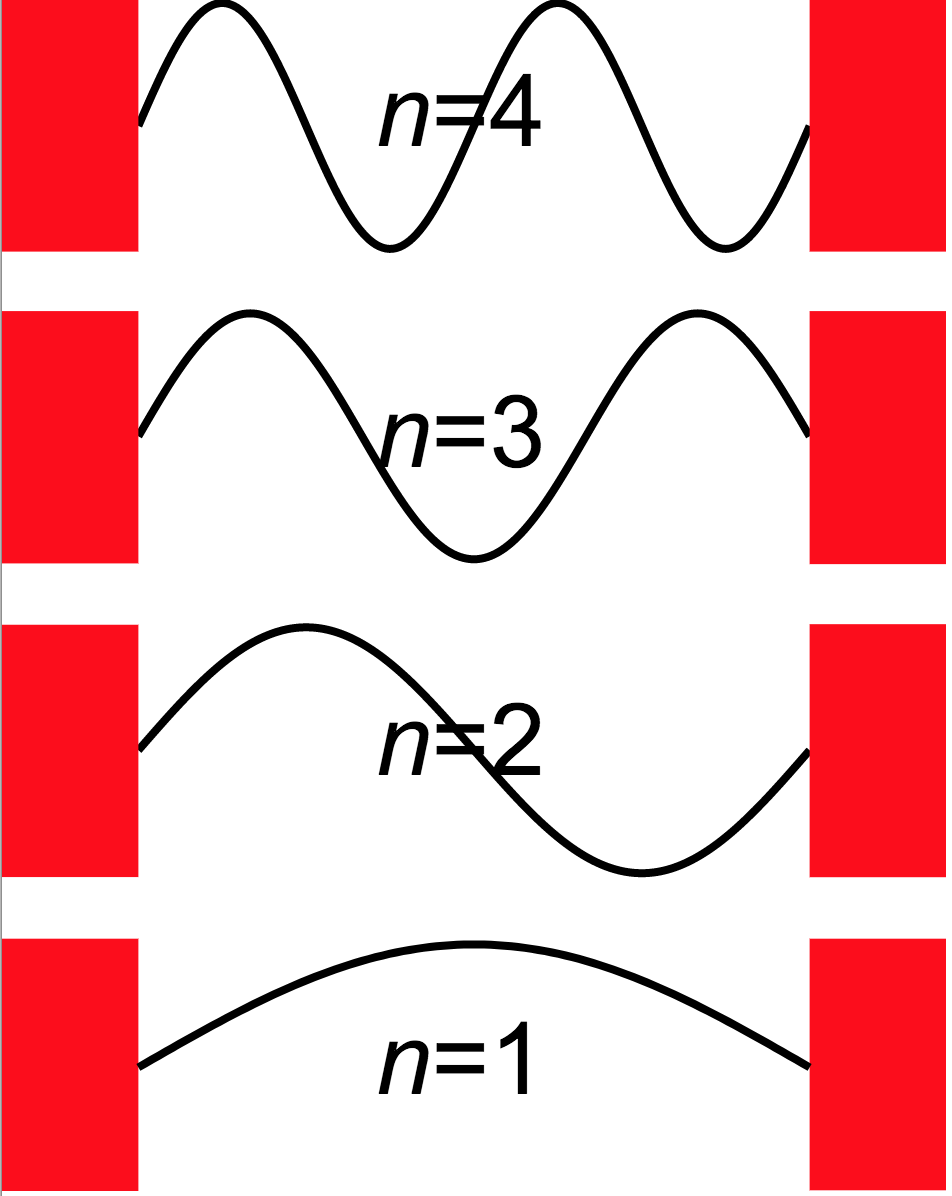
\includegraphics[scale=0.3]{ParticulaCaixa2.png}
\caption{Funcions d'ona corresponents als primers nivells d'energia d'una partícula en una caixa unidimensional.}
\label{fig:ParticulaCaixa2}
\end{figure}
De l'exemple de la partícula en una caixa podem extreure'n conceptes generals que ens serviran més endavant:
\begin{itemize}
\item Els nivells d'energia quantitzats només apareixen si confinem la partícula entre dos extrems de potencial infinit. Sempre que tinguem moviments confinats o periòdics, apareixerà quantització, com en la rotació d'una molècula.
\item A mesura que augmenta la massa de la partícula o disminueix l'espai en el què aquesta està confinada, la distància entre les energies de quantització es fa menor.
\item El fet que la funció d'ona passi de valors positius a negatius implica que hi ha punts en els quals el seu valor és zero (i que anomenem \textit{nodes}). En aquests punts, el seu quadrat també serà zero, i per tant la probabilitat de trobar-hi la partícula serà nul·la.
\end{itemize}
\section{L'àtom d'hidrogen}

\subsection{Números quàntics}
Estudiar l'àtom d'hidrògen, l'exemple més simple possible, ens permetrà comprendre la base de l'enllaç químic entre àtoms.
L'aplicació de l'equació de Schrödinger 
\begin{equation}
H\Psi = E\Psi
\label{Eq:Schr}
\end{equation}a aquest àtom dóna resultats que estan d'acord amb les dades experimentals que se'n tenen.
L'equació de Schrödinger té la virtut de no necessitar postular els números que descriuen la quantització de l'energia, com succeïa en el model de Bohr. A partir d'aquesta equació, els números de la quantització de l'energia sorgeixen de forma natural en solucionar-la. En el cas de l'àtom d'hidroegn, els números quàntics que sorgeixen són:
\begin{description}
\item[Número quàntic principal, $n$]  Determina les energies accessibles per l'àtom d'hidrogen o per qualsevol altre àtom d'un sol electró i càrrega nuclear $Z$:
\[
E=-\frac{2\pi^2 me^4 Z^2}{n^2 h^2}
\]
$n=1,2,3\ldots$
Aquest resultat s'obté de la resolució de l'Eq. \ref{Eq:Schr} i és el mateix que va trobar Bohr en el seu model.
Cal fixar-se que l'energia en un àtom d'hidrogen o en qualsevol àtom en el qual només hi hagi un electró només depèn del número atòmic $n$.
\item[Número quàntic del moment angular, $l$] En estar relacionat amb el moment angular de l'electró, també ho està amb la seva energia cinètica i, per tant, és lògic que estigui limitat pel valor de $n$ (que expressa els nivells permesos d'energia total). $l=0, 1, \ldots, n-1$.
\item[Número quàntic magnètic, $m_l$] Pel fet que un electró amb un determinat moment angular pot ser considerat com un corrent elèctric que cirsula en un anell, pot generar un camp magnètic associat a aquest corrent. Aquest camp magnètic, pel fet d'estar associat al moment angular, estarà limitat al valor d'$l$: $m_l=-1, -l+1, \ldots, 0, 1, \ldots, l-1,l$.
\item[Número quàntic d'spin, $m_s$] Mostra la propietat magnètica intrínseca de l'electró i la possibilitat de girar sobre el seu eix en un sentit o un altre: $m_s=\{+\frac{1}{2},-\frac{1}{2}\}$.
\end{description}

\section{Orbitals moleculars}
El nivell d'energia $n$ determina les possibilitats dels altres números. Per exemple, en l'estat fonamental, l'àtom d'hidrogen pot tenir les combinacions de $\{n,l,m_l,m_s\}$ $\{1,0,0,+\frac{1}{2}\}$ i $\{1,0,0,-\frac{1}{2}\}$. De la mateixa manera, podem pensar en els estats excitats de l'àtom d'hidrogen considerant altres valors dels números quàntics, de manera que anem determinant els diversos orbitals :
\begin{table}[h!]
  \begin{center}
    \caption{Números quàntics i orbitals \cite{mahan_quimico_1977}}
    \label{tab:quant}
    \begin{tabular}{cccccc}
      \hline
      $n$ & $l$ & Orbital & $m_l$ & $m_s$ & combinacions\\
      \hline
      1 & 0 & 1s & 0 & $+\frac{1}{2},-\frac{1}{2}$ & 2 \\
      2 & 0 & 2s & 0 & $+\frac{1}{2},-\frac{1}{2}$ & 2 \\
      2 & 1 & 2p & $+1,0,-1$ & $+\frac{1}{2},-\frac{1}{2}$ & 6 \\
      3 & 0 & 3s & 0 & $+\frac{1}{2},-\frac{1}{2}$ & 2 \\
      3 & 1 & 3p & $+1,0,-1$ & $+\frac{1}{2},-\frac{1}{2}$ & 6 \\
      3 & 2 & 3d & $+2,+1,0,-1,-2$ & $+\frac{1}{2},-\frac{1}{2}$ & 10 \\
      4 & 0 & 4s & 0 & $+\frac{1}{2},-\frac{1}{2}$ & 2 \\
      4 & 1 & 4p & $+1,0,-1$ & $+\frac{1}{2},-\frac{1}{2}$ & 6 \\
      4 & 2 & 4d & $+2,+1,0,-1,-2$ & $+\frac{1}{2},-\frac{1}{2}$ & 10 \\
      4 & 3 & 4f & $+3,+2,+1,0,-1,-2,-3$ & $+\frac{1}{2},-\frac{1}{2}$ & 14 \\
      \hline
    \end{tabular}
  \end{center}
\end{table}

Per a un interessant i complet resum d'aquest capítol, ves a \linkurl{https://2012books.lardbucket.org/books/principles-of-general-chemistry-v1.0/s10-05-atomic-orbitals-and-their-ener.html}.
\begin{figure}[h]
\centering
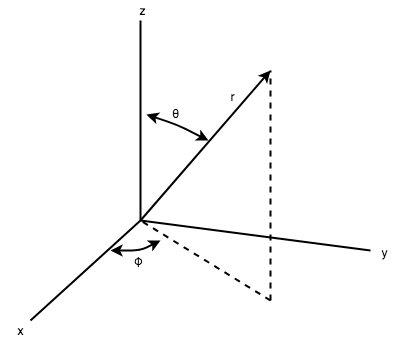
\includegraphics[scale=0.4]{SphericalCoords.png}
\caption{Coordenades esfèriques.}
\label{fig:SphericalCoords}
\end{figure}
A partir de la probabilitat de trobar un electró en un punt de l'espai, que ve donat per $\|\psi^2\|=1$ podem trobar la forma de les regions que ocuparà per a cada orbital (per analogia a les òrbites del model de Bohr). Si les expressem en coordenades esfèriques (Figura \ref{fig:SphericalCoords}) les funcions d'ona corresponents a cada orbital es poden expressar com a producte d'una part angular $\xi$ i una radial $R$ (veure Taula \ref{tab:AngRadOrb}).
\begin{equation}
\psi(r,\theta,\phi)=R_{n,l}(r)\chi_{l,m}(\theta,\phi)=R(r)\chi(\theta,\phi)
\label{Eq:psisplit}
\end{equation}
\begin{table}[h!]
  \begin{center}
    \caption{Part radial i part angular  de les funcions d'ona de l'àtom d'hidrogen \cite{mahan_quimico_1977}. $a=0$ és el radi de Bohr, $0.529 \times 10^{-10}$m.}
    \label{tab:AngRadOrb}
    \begin{tabular}{cc}
      \hline
      $\chi(\theta,\phi)$ & $R(r)$ \\
      \hline
      $\chi(s)=\left(\frac{1}{4\pi}\right)^{1/2}$ & $R(1s)=2 \left(\frac{Z}{a_0}\right)^{3/2} e^{-\sigma/2}$ \\
      \hline
$\begin{array}{rcl}
\chi (p_x)&=&\left(\frac{3}{4\pi}\right)^{1/2}\sin \theta \cos \phi \\
\chi (p_y)&=&\left(\frac{3}{4\pi}\right)^{1/2}\sin \theta \sin \phi \\
\chi (p_z)&=&\left(\frac{3}{4\pi}\right)^{1/2}\cos \theta 
\end{array}$
&
$\begin{array}{rcl}
R(2s) &=& \frac{1}{2\sqrt{2}}\left(\frac{Z}{a_0}\right)^{3/2} (2-\sigma) e^{-\sigma/2} \\
R(2p) &=& \frac{1}{2\sqrt{6}}\left(\frac{Z}{a_0}\right)^{3/2} \sigma e^{-\sigma/2} 
\end{array}$\\
      \hline
      $\begin{array}{rcl}
\chi (d_{z^2})&=&\left(\frac{5}{16\pi}\right)^{1/2} (3 cos^2 \theta -1) \\
\chi (d_{xz})&=&\left(\frac{15}{4\pi}\right)^{1/2}\sin \theta cos \theta \cos \phi \\
\chi (d_{yz})&=&\left(\frac{15}{4\pi}\right)^{1/2}\sin \theta cos \theta \sin \phi \\
\chi (d_{x^2-y^2})&=&\left(\frac{15}{4\pi}\right)^{1/2} \sin^2 \theta \cos 2\phi \\
\chi (d_{xy})&=&\left(\frac{15}{4\pi}\right)^{1/2} \sin^2 \theta \sin 2\phi \\
\end{array}$
&
$\begin{array}{rcl}
R(3s) &=& \frac{1}{9\sqrt{3}}\left(\frac{Z}{a_0}\right)^{3/2} (6-6\sigma +\sigma^2) e^{-\sigma/2} \\
R(3p) &=& \frac{1}{9\sqrt{6}}\left(\frac{Z}{a_0}\right)^{3/2} \sigma (4-\sigma) \sigma e^{-\sigma/2} \\
R(3d) &=& \frac{1}{9\sqrt{30}}\left(\frac{Z}{a_0}\right)^{3/2} \sigma^2 e^{-\sigma/2} 
\end{array}$\\
      \hline
      & $\sigma=\frac{2Zr}{na_0}; \; a_0=\frac{h^2}{4\pi^2 m e^2}$\\
      \hline
    \end{tabular}
  \end{center}
\end{table}

A partir de la Taula \ref{tab:AngRadOrb} es poden obtenir les funcions d'ona de tots els orbitals de l'àtom d'hidrogen. Per exemple, per a l'orbital 1s tenim:
\[
\psi(1s)= \frac{1}{\pi^{1/2}} \left( \frac{Z}{a_0} \right)^{3/2} e^{-Zr/a_0}
\]
i dóna una probabilitat de trobar l'electró a una distància $r$ de
\[
\psi^2(1s)= \frac{1}{\pi} \left( \frac{Z}{a_0} \right)^{3} e^{2Zr/a_0}
\]
que mostra com, en un orbital 1s, la màxima probabilitat de trobar l'electró es dóna a prop del nucli, i és independent de l'angle. 

\begin{exr}
Quants nodes té la funció $\psi(2s)$? i la $\psi(3s)$? i la $\psi(2p)$? 
\end{exr}
Com a norma, el número de nodes que podem trobar és $n-1-l$. 
En afegit, i per entendre millor la distribució electrònica, podem pensar en la densitat de probabilitat radial.
Aquesta es calcula trobant, a partir de la integració de l'expressió \ref{Eq:psisplit}, la probabilitat de trobar l'electró en un àtom hidrogenoïde (un sol electró), a una distància $r$ del nucli entre $r$ i $r+dr$, amb un angle $\theta$ entre $\theta$ i $\theta+d\theta$, i un angle $\phi$ entre $\phi$ i $\phi+d\phi$:
\[
|\psi(r,\theta,\phi)| d\tau = [R(r)]^2 [\chi(\theta,\phi)]^2 r^2 \sin \theta dr d\theta d\phi
\]
Integrant per als angles trobem la distribució radial:
\[
D(r)dr=r^2[R(r)]^2 dr \underbrace{\int_0^{\pi} \int_0^{2\pi} [\chi(\theta,\phi)]^2 \sin \theta dr d\theta d\phi}_{=1}=r^2[R(r)]^2 dr
\]
\begin{exr}
A partir de la densitat de probabilitat podem preguntar-nos coses com on és el màxim de probabilitat (solucionant  $\frac{d D(r)}{dr}=0$) o bé calculant el valor promig de la distància de l'electró al nucli segons $<r>_{n,l}=\int_0^{\infty} r D(r)dr$. Mostra que $<r>_{2s}=\frac{6a_0}{Z}$ i $<r>_{2p}=\frac{5a_0}{Z}$ (veure Figura \ref{fig:D2s2p}).\footnote{https://chemistry.stackexchange.com/questions/15208/difference-between-actual-position-of-electron-and-radial-distribution-probabili}
\end{exr}
\begin{figure}[h]
\centering
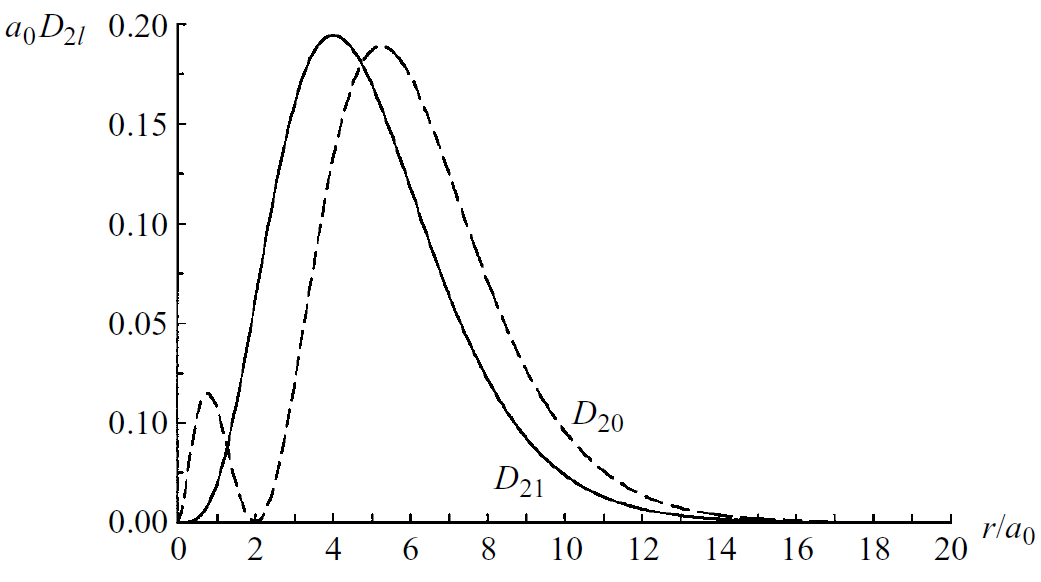
\includegraphics[scale=0.35]{D2s2p.png}
\caption{Funció de distribució radial $D(r)$ per a les funcions 2s i 2p}
\label{fig:D2s2p}
\end{figure}
Per a cada combinació de números quàntics tenim resultats diferents (veure \linkurl{http://hyperphysics.phy-astr.gsu.edu/hbase/hydwf.html} i Figura \ref{fig:Hydrogen_Density_Plots}).


\begin{figure}[h]
\centering
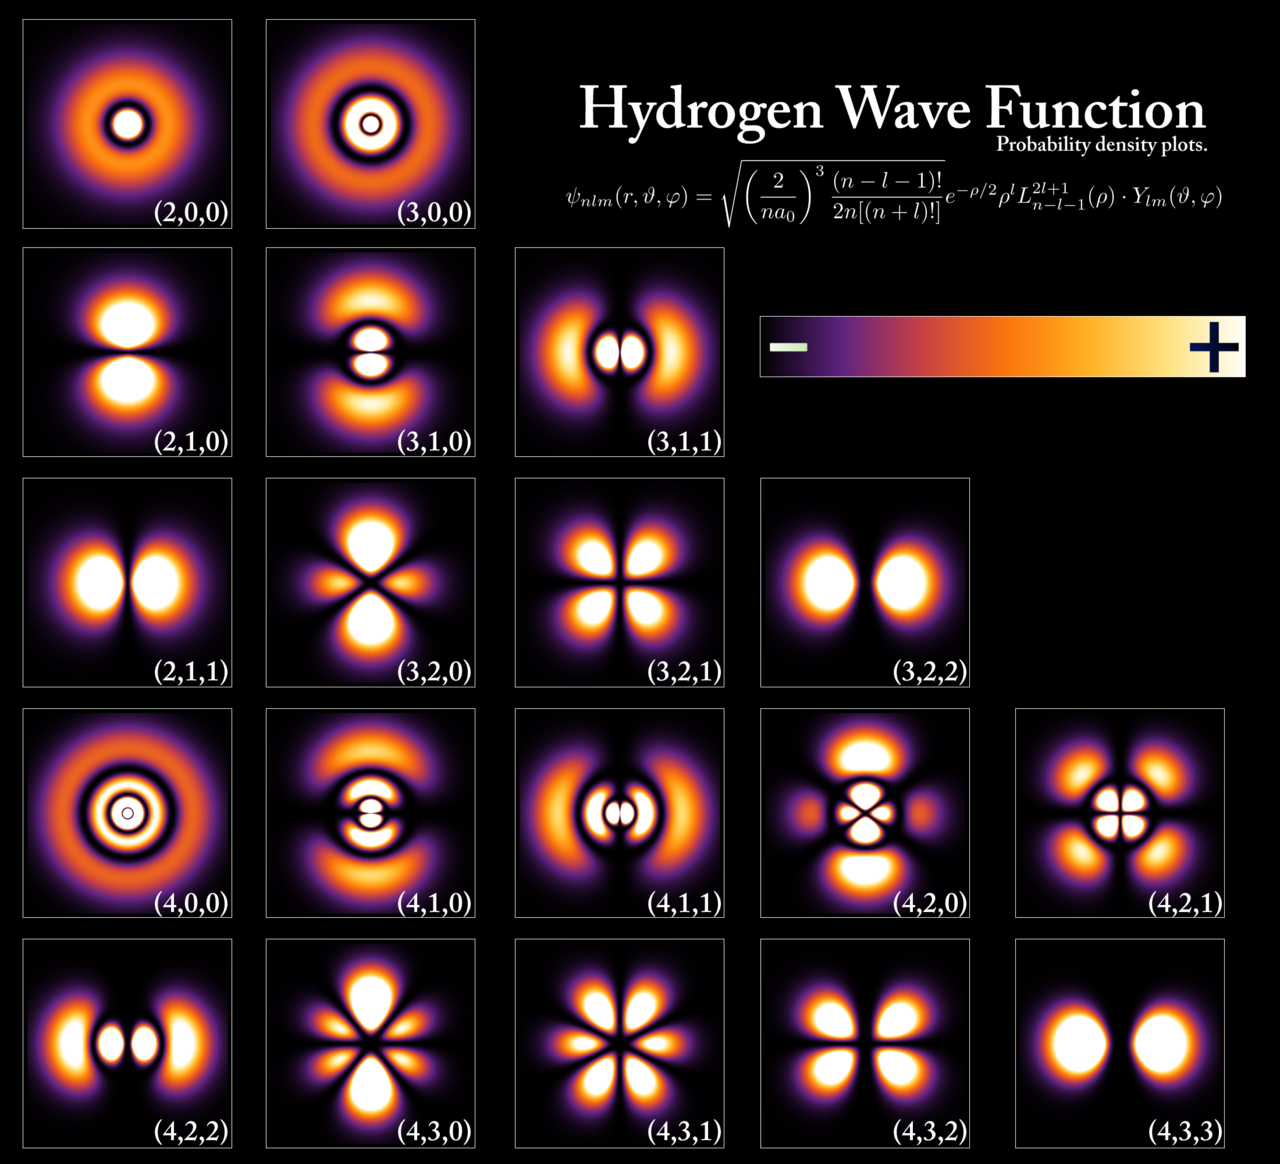
\includegraphics[scale=0.25]{Hydrogen_Density_Plots.png}
\caption{Densitat electrònica dels diferents orbitals de l'hidrogen}
\label{fig:Hydrogen_Density_Plots}
\end{figure}



%Això ens permetrà  entendre, entre altres efectes, la manera en què els complexes organometàl·lics es formen (Figura \ref{fig:coordination}).
%\begin{figure}[h]
%\centering
%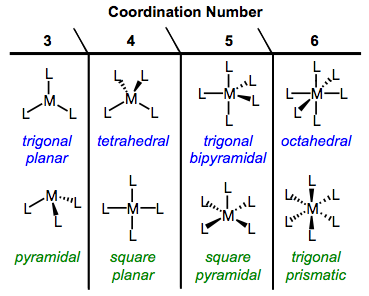
\includegraphics[scale=0.35]{coordination.png}
%\caption{Coordinació en complexes organometàl·lics}
%\label{fig:coordination}
%\end{figure}



\section{Propietats periòdiques}

Quan analitzem els orbitals de l'àtom d'hidrogen (o d'àtoms hidrogenoïdes, amb un sol electró), i en tant que la seva energia només depèn del número quàntic principal $n$, diem que són degenerats. En el cas d'àtoms polielectrònics, l'apantallament dels electrons interns fa que aquesta degeneració desaparegui. En realitat, el que succeeix és que l'aproximació de parlar d'orbitals atòmics com en el cas de l'hidrogen ja no és vàlida i és només una aproximació, en tant que l'equació d'Schrödinger ja no es pot resoldre en aquests àtoms.
Sigui com sigui, la Figura \ref{fig:degeneracio} mostra l'efecte en l'energia dels orbitals atòmics de tenir més d'un electró en l'àtom.
\begin{figure}[h]
\centering
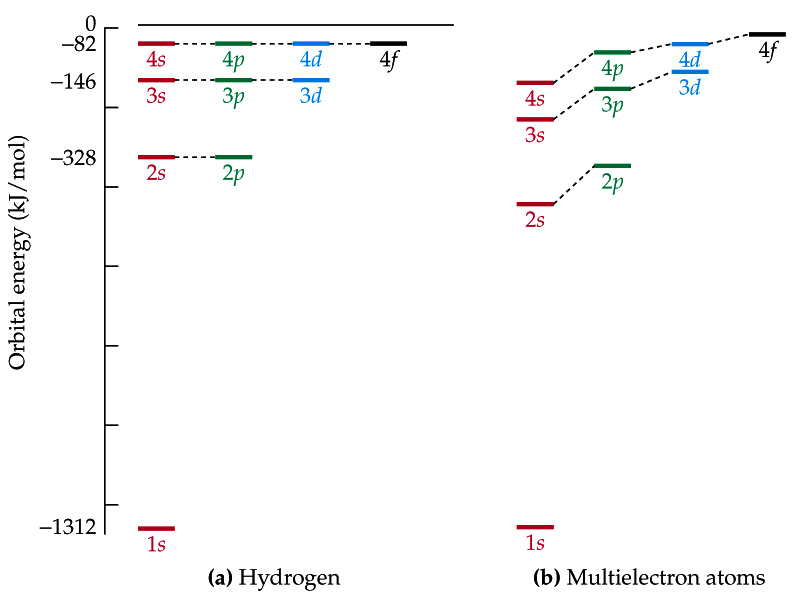
\includegraphics[scale=0.35]{degeneracio.png}
\caption{Degeneració dels orbitals de l'àtom d'hidrogen i d'àtoms polielectrònics}
\label{fig:degeneracio}
\end{figure}

El principi d'exclusió de Pauli determina que no hi poden haver dos electrons amb els mateixos números quàntics. Per tant, a cada orbital atòmic només hi poden haver dos electrons, amb $m_s=1/2$ i $m_s=-1/2$.
\begin{exr}
L'àtom de sodi es comporta de forma similar a l'àtom d'hidrogen pel que fa a la seva facilitat de "donar" un electró. Ho pots explicar en base a les densitats de probabilitat explicades a l'apartat anterior? Pensa en la llei de Coulomb i l'efecte pantalla dels electrons interiors.
\end{exr}
\begin{exr}
Escriu la configuració electrònica de l'argó i del potassi. Perquè després d'omplir els orbitals 3p no omplim els orbitals 3d? Com raones que els metalls de transició de les  darreres columnes de la taula periòdica tinguin típicament valències de +2?
\end{exr}
\begin{exr}
Pots explicar les dades de la Figura \ref{fig:AfinitatElectronica} en base a la configuració electrònica dels elements representats?
\end{exr}
\begin{figure}[h]
\centering
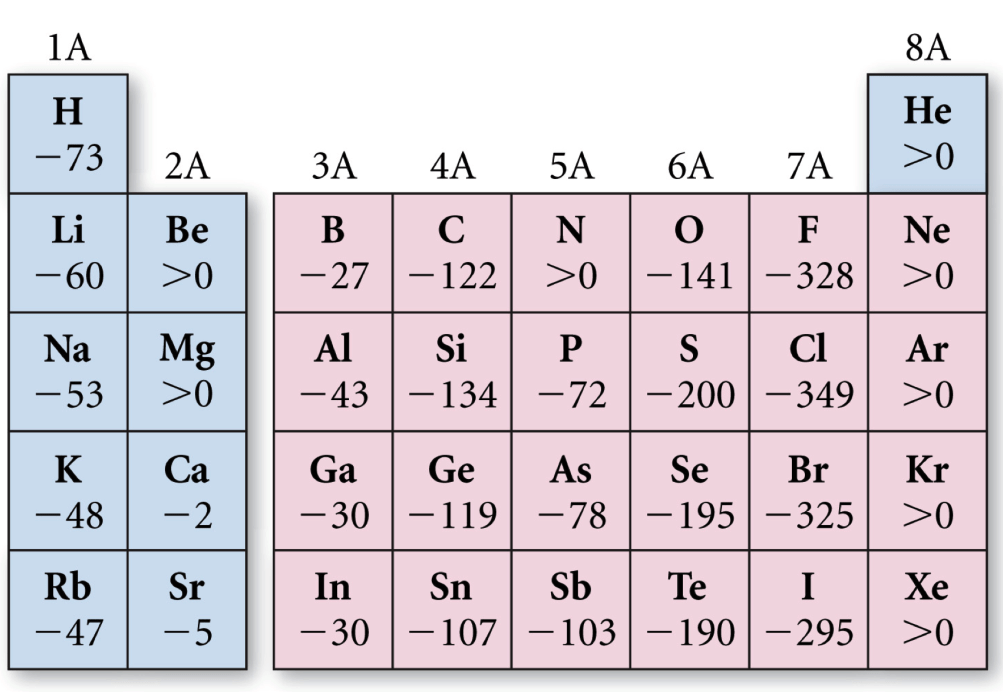
\includegraphics[scale=0.5]{AfinitatElectronica.png}
\caption{Afinitat electrònica de diversos elements de la taula periòdica}
\label{fig:AfinitatElectronica}
\end{figure}
